\clearpage
\section{Selectivity and Optimization Principle}
\subsection{Question (Paper \& Pencil)} 
\label{sec:obj_fcn}
We can write the gradient descent on the objective function F($\omega$) as:
\begin{eqnarray}
\Delta \omega&=&\eta \frac{\partial F(\omega)}{\partial \omega} \\
&\approx&\frac{\partial }{\partial \omega} \left\langle \left(\frac{y}{\sigma_y}\right)^3 \right\rangle \\
&\approx&\frac{\partial }{\partial \omega} \left\langle \left(\frac{y}{\sqrt{\langle y^2\rangle}}\right)^3 \right\rangle \\
&\approx&\frac{\partial }{\partial \omega} \left\langle \frac{y^3}{\langle y^2\rangle  \sqrt{\langle y^2\rangle}} \right\rangle
\end{eqnarray}

using the given $\sigma_y = \sqrt{\langle y^2\rangle}$. Using the distributive properties of the expectation operation (i.e. $\langle A + B \langle C\rangle\rangle = \langle A  \rangle + \langle B\rangle \langle C\rangle$ and $\left\langle \frac{A}{\langle B\rangle}\right\rangle = \frac{\langle A  \rangle}{\langle B  \rangle}$ we can write Eq. \ref{eq:distri}: 

\begin{eqnarray}
\Delta \omega&\approx& \frac{\partial }{\partial \omega}  \frac{\langle y^3 \rangle}{\langle y^2 \rangle \langle \sqrt{\langle y^2 \rangle}\rangle}  \label{eq:distri}\\
\end{eqnarray}

and knowing $\theta = \frac{\langle y^3\rangle}{\langle y^2\rangle}$, 
\begin{eqnarray}
\Delta \omega&\approx& \frac{\partial }{\partial \omega}  \frac{\theta}{ \langle \sqrt{\langle y^2 \rangle}\rangle} \\
\end{eqnarray}

taking the derivative yields: 
\begin{eqnarray}
\Delta \omega&\approx& \frac{\partial \theta}{\partial \omega}  \frac{1}{ \langle \sqrt{\langle y^2 \rangle}\rangle} -  \frac{\theta}{2}  {\langle y^2 \rangle}^{-3/2} \langle 2y x \rangle \label{eq:delta_omega}
\end{eqnarray}

now noticing $\langle {\langle y^2 \rangle}^{1/2} \rangle$ has an outer expectation value operation on a scalar, we can write $ {\langle y^2 \rangle}^{1/2} $ instead.

Partial derivative of $\theta$ with respect to $\omega$:

\begin{eqnarray}
\frac{\partial \theta}{\partial \omega} &=& \frac{\langle 3y^2 x\rangle}{\langle y^2 \rangle}  - \frac{\langle y^3\rangle}{\langle y^2\rangle^2} \langle 2yx\rangle \\
 &=& \frac{3\langle y^2 x\rangle}{\langle y^2 \rangle}  - \frac{\theta}{\langle y^2\rangle} 2\langle yx\rangle \\
 &=& \frac{3\langle y^2 x\rangle-2\theta\langle yx\rangle}{\langle y^2 \rangle}  \label{eq:partial_theta}
\end{eqnarray}

If we use Eq. \ref{eq:partial_theta} in Eq. \ref{eq:delta_omega}, we get: 
\begin{eqnarray}
\Delta \omega&\approx&  \frac{3\langle y^2 x\rangle-2\theta\langle yx\rangle}{\langle y^2 \rangle^{3/2}}   -  \frac{\theta \langle y x \rangle}  {\langle y^2 \rangle^{3/2}} \\
\Delta \omega&\approx&  3\frac{\langle y^2 x\rangle-\theta\langle yx\rangle}{\langle y^2 \rangle^{3/2}}  \label{eq:final_form} 
\end{eqnarray}

where Eq. \ref{eq:final_form} is of the form $\dot\omega =  xy^2 - xy\theta$.
\newpage
\subsection{Question (Simulation)}
In this section, 30 independent experiments were run with different initialization of $\omega_o$. We see that after learning takes place for a sufficiently long time, the weights to the postsynaptic neuron corresponding to the input Gaussian patterns strengthen. Fig. \ref{fig:weights_converged} shows maximum strengthening around neurons $10, 30, 50, 70$ and $ 90$, corresponding respectively to the maxima of the input. This demonstrates the selectivity of these neurons to the input patterns presented at random. Differences in amplitude of the weights is thought to be an artifact of the frequency at which the random input patterns were selected.   



\begin{figure}[h]
\centering
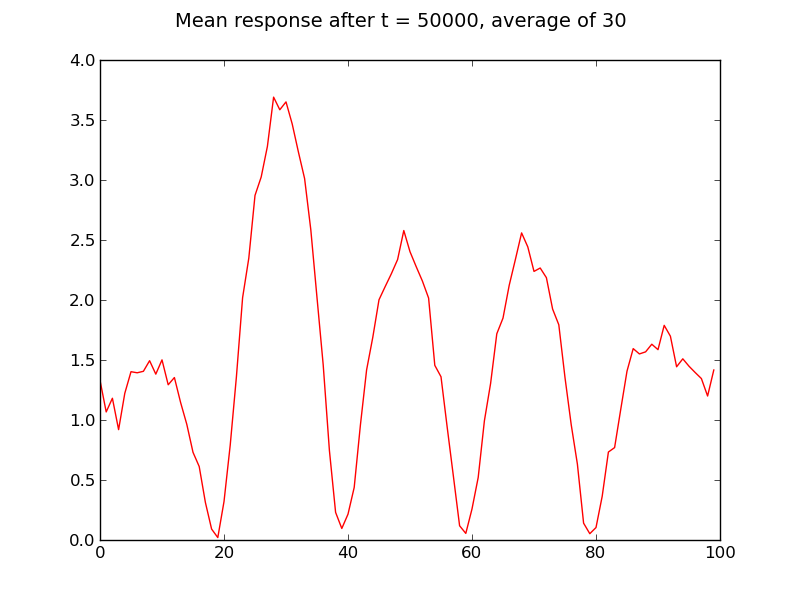
\includegraphics[width=0.7\textwidth]{../ex2/weights_t50000_mean_results.png}
\caption{Converged weights for all input neurons.}
\label{fig:weights_converged}
\end{figure}

In Fig. \ref{fig:theta_over_time}, we see that the threshold $\theta$ first decreases and then increases until it converges to a stable value. From the differential equations in Question 1 we would expect an exponential decay, and convergence to $\langle y^2\rangle$.

\begin{figure}[h]
\centering
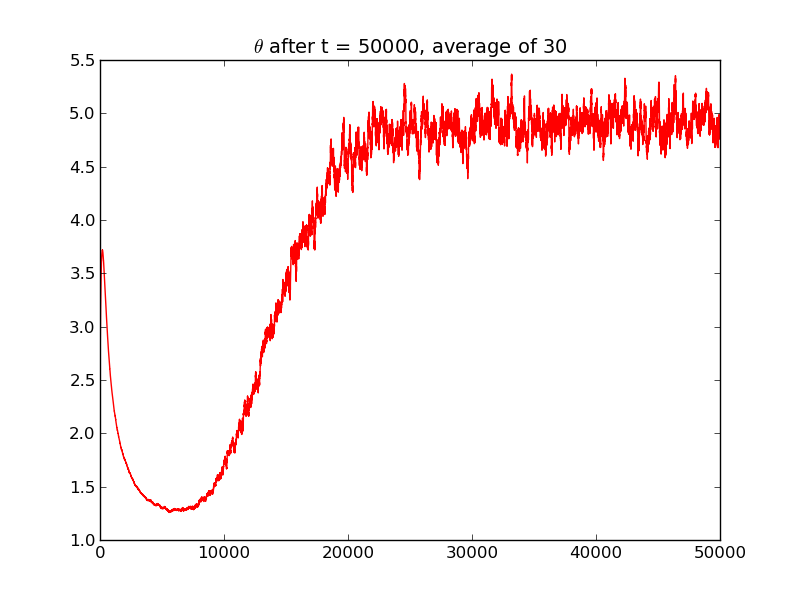
\includegraphics[width=0.7\textwidth]{../ex2/theta_t50000_mean_results.png}
\caption{Evolution of $\theta (t)$ over time.}
\label{fig:theta_over_time}
\end{figure}
In Fig. \ref{fig:response_over_time}, we see that $\langle y\rangle$ decreases until it converges to a stable value. The reponse should stabilize with convergence, as seen in this figure. 
\begin{figure}[h]
\centering
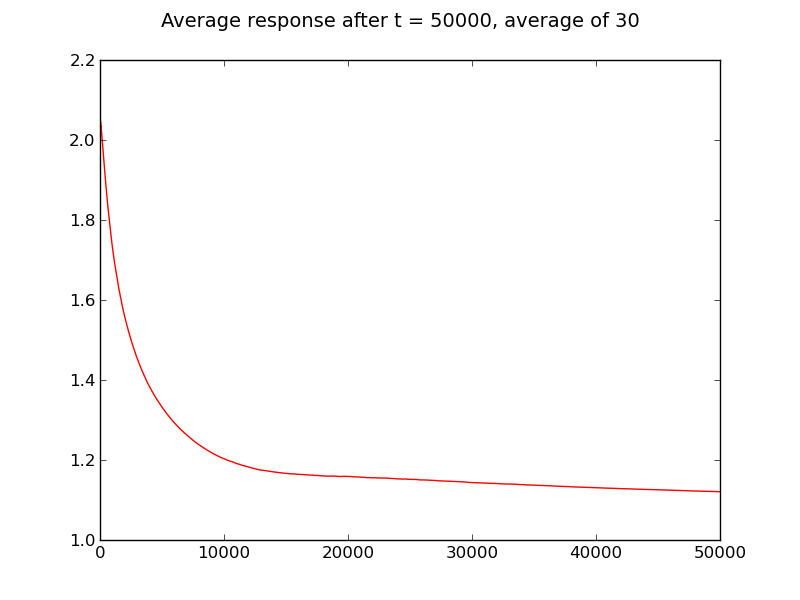
\includegraphics[width=0.7\textwidth]{../ex2/resp_avg_t50000_mean_results.png}
\caption{Evolution of the averaged response $\langle y\rangle$ over time.}
\label{fig:response_over_time}
\end{figure}

Fig. \ref{fig:obj_over_time} shows a drop followed by a rise in the objective function $F(\omega)$. Recalling that in Part. \ref{sec:obj_fcn} gradient descent on $F(\omega)$ gave us the BCM-like learning rule, we should see that if we use the BCM learning rule, we get a decrease in the objective function. 
\begin{figure}[h]
\centering
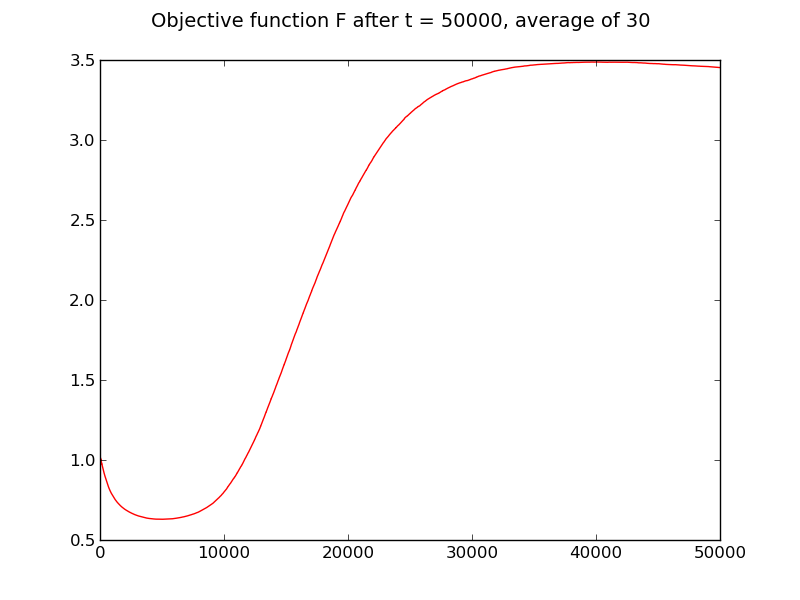
\includegraphics[width=0.7\textwidth]{../ex2/obj_t50000_mean_results.png}
\caption{Evolution of the objective function $F(\omega)$ over time.}
\label{fig:obj_over_time}
\end{figure}

